\section{Introduction}
% \label{sec:introduction}
% \textcolor{blue}{Skeleton of intro: OT and its application $\implies$ Yet OT requires stringent requirement on balanced masses $\to$ impractical. Then discuss and cite other unbalanced OT variants. Among them, POT is the BEST, since a, b, c.}
Optimal Transport (OT) \cite{Villani-09-Optimal, Kantorovich-1942-Translocation}, which seeks a minimum-cost coupling between two balanced measures, is a well-studied topic in mathematics and operations research. With the introduction of entropic regularization  \cite{Cuturi-2013-Sinkhorn}, the scalability and speed of OT computation have been significantly improved, facilitating its widespread applications in machine learning such as domain adaptation \citep{Courty-2017-Optimal}, and dictionary learning \citep{pmlr-v51-rolet16}. 
However, OT has a stringent requirement that the input measures must have equal total masses  \citep{Chizat_2015}, hindering its practicality in various other machine learning applications, which require an optimal matching between two measures with unbalanced masses, such as averaging of neuroimaging data \citep{Gramfort_2015} and image classification \citep{Pele2008ALT, rubner2000earth}.

% generative adversarial networks \citep{Salimans_2018}
% Two alternatives to OT have been developed in response to this limitation. The first alternative, Unbalanced Optimal Transport (UOT), regularizes the objective by penalizing the marginal constraints via some given divergences \citep{UOT_complexity, Liero_Optimal_2018} including Kullback-Leiber \citep{chizat2017scaling} or squared $\ell_2$ norm \citep{Blondel-2018-Smooth}. Several works have studied UOT both in terms of computational complexity \citep{UOT_complexity, gem-uot} and applications \citep{Janati_Wasserstein_2019, balaji2020robust, Yang_Scalable_2019}. \textcolor{red}{We don't have to mention UOT}
In response to such limitations, Partial Optimal Transport (POT), which explicitly constrains the mass to be transported between two unbalanced measures, was proposed. It has been studied from the perspective of partial differential equations by theorists \cite{figalli2010optimal, Caffarelli_2010}. Practically, the relaxation of the marginal constraints, which are strictly imposed by the standard OT, and the control over the total mass transported grant POT immense flexibility compared to OT \citep{Chapel-nips2020} and more robustness to outliers \citep{nhatho-mmpot}. POT has been deployed in various recent AI applications such as color transfer \citep{Bonneel_2019}, graph neural networks \citep{Sarlin_2019}, graph matching \cite{Liu_2020},  partial covering \citep{Kawano_2021}, point set registration \citep{Wang_2022}, and robust estimation \citep{nietert2023robust}.   

% Aside from classical tasks in computer vision \citep{Pele2008ALT, rubner2000earth},
% positive-unlabeled learning \citep{Chapel-nips2020},
% Despite its applicability, POT faces a computation bottleneck due to its more intricate structural constraints imposed on admissible couplings.
% %have hindered the direct adaptation of any efficient OT solver in the literature.
% Currently, the literature \citep{Chapel-nips2020, nhatho-mmpot} relies on reformulating POT as an extended OT problem under additional assumptions on the input masses. The OT problem can then be solved via existing methods such as Sinkhorn \citep{nhatho-mmpot}, and its solution can be converted back to an admissible POT coupling.
% % which can then be solved via existing methods for computing OT, and finally retrieve an admissible POT coupling from the solution to the extended OT problem.

Despite its potential applicability, POT still suffers from the computation bottleneck, whereby the more intricate structural constraints imposed on admissible couplings have hindered the direct adaptation of any efficient OT solver in the literature. Currently, the literature \citep{Chapel-nips2020, nhatho-mmpot} relies on reformulating POT into an extended OT problem under additional assumptions on the input masses, which can then be solved via existing OT methods, and finally retrieves an admissible POT coupling from the solution to the extended OT problem. This approach has two fundamental drawbacks. First, in the reformulated OT problem, the maximum entry of the extended cost matrix is increased \citep[Proposition 1]{Chapel-nips2020}, which will always worsen the computational complexity since most efficient algorithms for standard OT \citep{Dvurechensky-2018-Computational, lin2019efficient, guminov2021accelerated} depend on this maximum entry in their complexities. 
Second, we discover, more details in the Revisiting Sinkhorn section, that although Sinkhorn for POT proposed by \citep{nhatho-mmpot} achieves the best known complexity of $\mathcal{\widetilde O}(n^2/\varepsilon^2)$, it in fact always outputs a \emph{strictly infeasible} solution to the POT problem. In brief, by discarding the last row and column of the reformulated OT solution obtained by Sinkhorn, the POT solution, transportation matrix $\vX$, will violate the equality constraint $\ones^\top \vX \ones = s$, which controls the total transported mass. Violating this equality constraint can degrade the results of practical applications in robust regimes such as point cloud registration \citep{qin2022rigid} and mini-batch OT \citep{nguyen2022improving} (refer to Remark \ref{remark:violation} and our Point Cloud Registration experiment). We theoretically justify the ungroundedness of Sinkhorn for POT in the Revisiting Sinkhorn section and empirically verify this claim in several applications in the Numerical Experiment section. Here, in Figure \ref{fig:Infeasible_Sinkhorn}, we specifically investigate Sinkhorn infeasibility in a color transfer example (detailed experimental setup in the later Numerical Experiment section). We show that the optimality gap produced by Sinkhorn is unable to reduce lower than $\varepsilon$, the tolerance of the problem (red line). In other words, Sinkhorn fails to produce an adequate $\varepsilon$-approximate POT solution. 

\begin{table*}[t]
    \centering
    \renewcommand\arraystretch{1.12}
    \begin{tabular}{c c c c}
        \toprule
        Algorithm & Regularizer & Cost per iteration & Iteration complexity \\
        \hline
        Iterative Bregman projections \cite{benamou2015iterative} & Entropic & Unspecified & Unspecified\\ %\footnote{$\omega(n^{2}/\varepsilon^2)$}
        (Infeasible) Sinkhorn \citep{nhatho-mmpot} & Entropic & $\mathcal{O}(n^2)$ & $\widetilde{\mathcal{O}}(1/\varepsilon^2)$\\
        (Feasible) Sinkhorn (\textbf{This paper}) & Entropic & $\mathcal{O}\br{n^2}$ & $\widetilde{\mathcal{O}}\br{1/\varepsilon^4}$ \\
        APDAGD (\textbf{This paper}) & Entropic & $\mathcal{O}(n^2)$ & $\widetilde{\mathcal{O}}\br{\sqrt{n}/\varepsilon}$ \\
        Dual Extrapolation (\textbf{This paper}) & Area-convex & $\mathcal{O}(n^2)$ & $\widetilde{\mathcal{O}}\br{1/\varepsilon}$\\
        \bottomrule
        \end{tabular}
    \caption{Type of regularizers and orders of complexity for four algorithms for POT approximation.} \label{Order_of_complexities}
\end{table*}

\begin{figure}
    \centering
    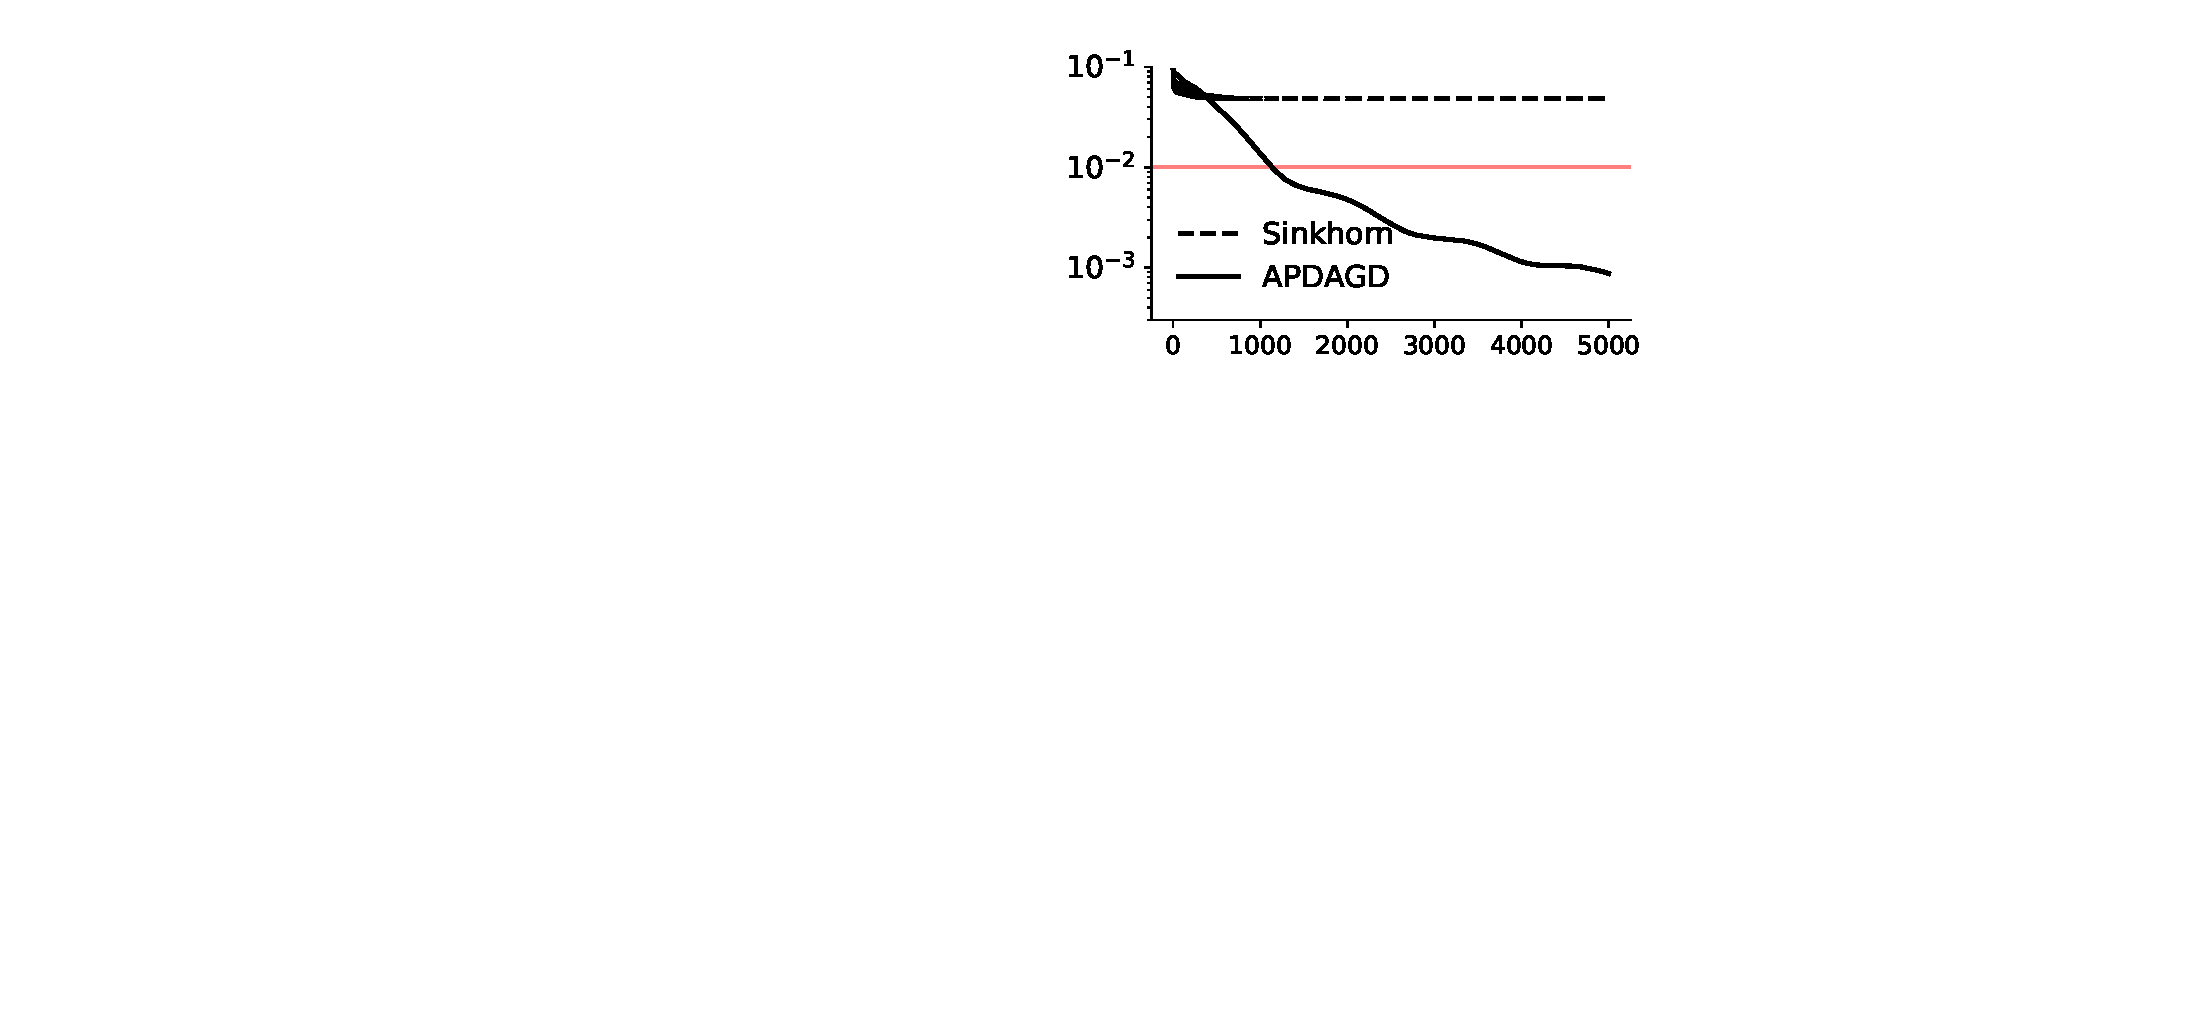
\includegraphics[width=0.8\linewidth]{figs/color_transfer_primal_opt.pdf}
    \caption{Primal optimality gap against optimization rounds achieved by Sinkhorn \cite{nhatho-mmpot} and APDAGD for POT. The marginal distributions are taken from a color transfer application described in our Numerical Experiments section, and the red horizontal line depicts the pre-defined tolerance ($\varepsilon$) for both algorithms.}
    \label{fig:Infeasible_Sinkhorn}
\end{figure}

To the best of our knowledge, the invalidity of Sinkhorn means there is currently no efficient method for solving POT in the literature. We attribute this to the fact that while the equivalence between POT and extended OT holds at optimality, all efficient OT solvers instead only output an approximation of the optimum value before projecting it back to the feasible set. However, the well-known rounding algorithm by \citep{altschuler2017near}, which is specifically designed for OT, does not guarantee to respect the more intricate structural constraints of POT, resulting in the invalidity of Sinkhorn. Motivated by this challenge and the success of optimization literature for OT, we raise the following central question of this paper: 
\begin{center}
\emph{Can we design a rounding algorithm for POT and then utilize it to develop efficient algorithms for POT that even match the best-known complexities of those for OT?} 
\end{center}
We affirmatively answer this question and formally summarize our contributions as follows.

\begin{itemize}
    \item We theoretically and experimentally show the infeasibility of the state-of-the-art Sinkhorn algorithm for POT  due to its incompatible rounding algorithm. We propose a novel POT rounding procedure \textsc{Round-POT} (Rounding Algorithm Section), which projects an approximate solution onto the feasible POT set in $\mathcal{O}(n^2)$ time. 
    \item From our theoretical bounds of the Sinkhorn constraint violations and the newly introduced \textsc{Round-POT}, we provide a revised procedure for Sinkhorn which will return a feasible POT solution. We also establish the revised complexity of Sinkhorn for POT (Table \ref{Order_of_complexities}).
    \item Predicated on our novel dual formulation for entropic regularized POT objective, our proposed Adaptive Primal-Dual Accelerated Gradient Descent (APDAGD) algorithm for POT finds an $\varepsilon$-approximate solution in  $\mathcal{\widetilde O}(n^{2.5}/\varepsilon)$, which is better in $\varepsilon$ than the revised Sinkhorn.  
    Various experiments on synthetic and real datasets and with applications such as point cloud registration, color transfer, and domain adaptation illustrate not only our algorithms' favorable performance against the pre-revised Sinkhorn but also the versatility of POT compared to OT. 
    \item Motivated by our novel rounding algorithm, we further reformulate the POT problem with $\ell_1$ penalization as a minimax problem and propose Dual Extrapolation (DE) framework for POT. We prove that DE algorithm can theoretically achieve $\mathcal{\widetilde O}(n^{2}/\varepsilon)$ computational complexity, thereby being the best in the POT literature to the best of our knowledge (Table \ref{Order_of_complexities}). 
\end{itemize}